\chapter{Resultaten} \label{ch:resultaten}
% Bespreking alle relevante grafieken
% wat zijn de eigenaardigheden
% bij de grafieken bespreken dat totaal niet echt totaal is voor de pi

In dit hoofdstuk zullen de resultaten besproken worden. We bespreken elke grafiek die gegenereerd wordt uit vorig hoofdstuk. We beginnen met eerst twee kanttekeningen te maken. De eerste kanttekening betreft het programma $Image~Recognition$ (Im Rec) uitgevoerd op de Raspberry Pi. De Pi kon voor dit programma geen resultaten halen. Het programma kon niet op betrouwbare manier herhaaldelijk uitgevoerd worden. Er zal dus op die locatie in de grafiek geen data aanwezig zijn. Dit heeft de tweede kanttekening als gevolg. In het totaal voor de Raspberry Pi zit de tijdswaarde van dit programma niet. Het totaal zal lager liggen dan als het programma wel uitgevoerd zou kunnen worden. Men kan dus niet het totaal van de Pi rechtstreeks vergelijken met het totaal van andere devices waar de tijdswaarde van Im Rec wel in verrekend zit.

\newpage

	\section{Ruwe benchmark gegevens}
	De eerste analyse behandelt de ruwe benchmark gegevens. Deze zijn terug te vinden in figuur \ref{fig:Figure_0} en \ref{fig:Figure_1} waarin respectievelijk de latency en \gls{cpu}-verbruik gegevens in worden weergegeven. In figuur \ref{fig:Figure_2} kan de genormaliseerde latencydata teruggevonden worden. Op de eerste figuur kan een duidelijk verschil tussen de edge-devices en de Personal Computer opgemerkt worden over alle programma's heen. De Personal Computer heeft telkens een beduidend lagere latency. Dit ligt in lijn met de stevigere hardware waar de Personal Computer over beschikt. 
	
	Als we de edge-devices met elkaar vergelijken op de figuur met genormaliseerde latencydata valt er ook een consistent verschil op te merken. Hier haalt de Jetson Nano bij zowel regressie als classificatie lagere tijdswaarden bij elk programma. De Coral Dev behaalt grotere latencies dan de Nano en bij de Pi duurt het uitvoeren van een programma altijd het langst. Er valt bij de regressieprogramma's ook een nagenoeg constante relatieve verhouding op te merken tussen alle devices. Tussen de Personal Computer en de Nano ligt dit rond de 6.2 die enkel bij het gradient-programma afwijkt. De verhouding van de Coral t.o.v. de Nano ligt rond 1.3 en dit blijft ook behouden bij de het gradient-programma. Tussen de Pi en de Coral ligt deze verhouding over de regressie programma's rond de 1.23. Bij de classificatieprogramma's vari\"eren deze verhoudingen veel meer. 
	
	



	\begin{figure}
		\makebox[\textwidth][c]{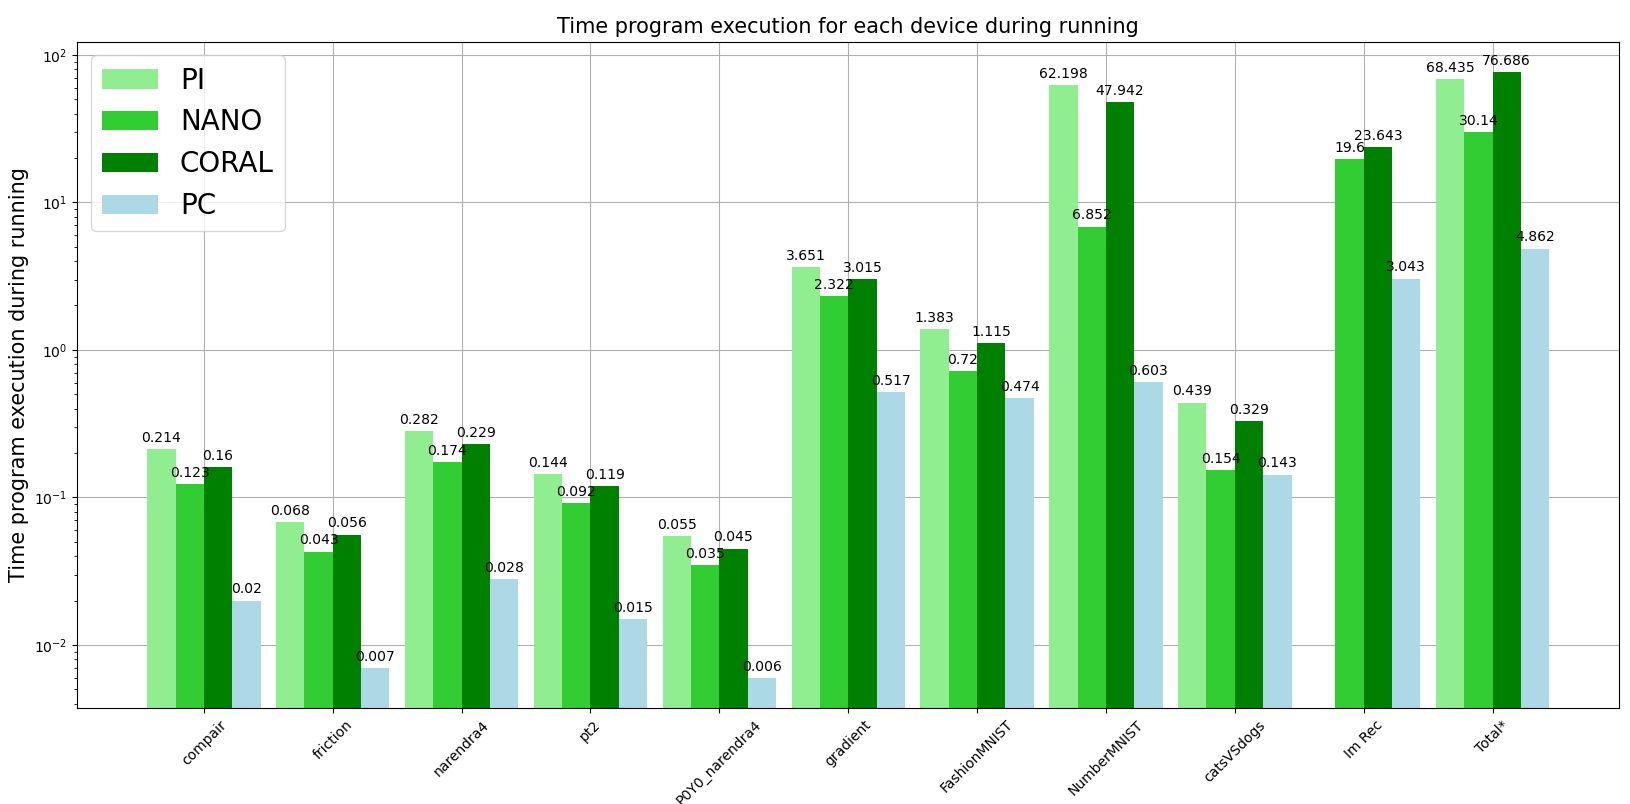
\includegraphics[width=1.25\textwidth]{afbeeldingen/Figure_0.png}}
		\caption{Staafdiagram met de latencydata.}
		\label{fig:Figure_0}
	\end{figure}

	\begin{figure}
		\makebox[\textwidth][c]{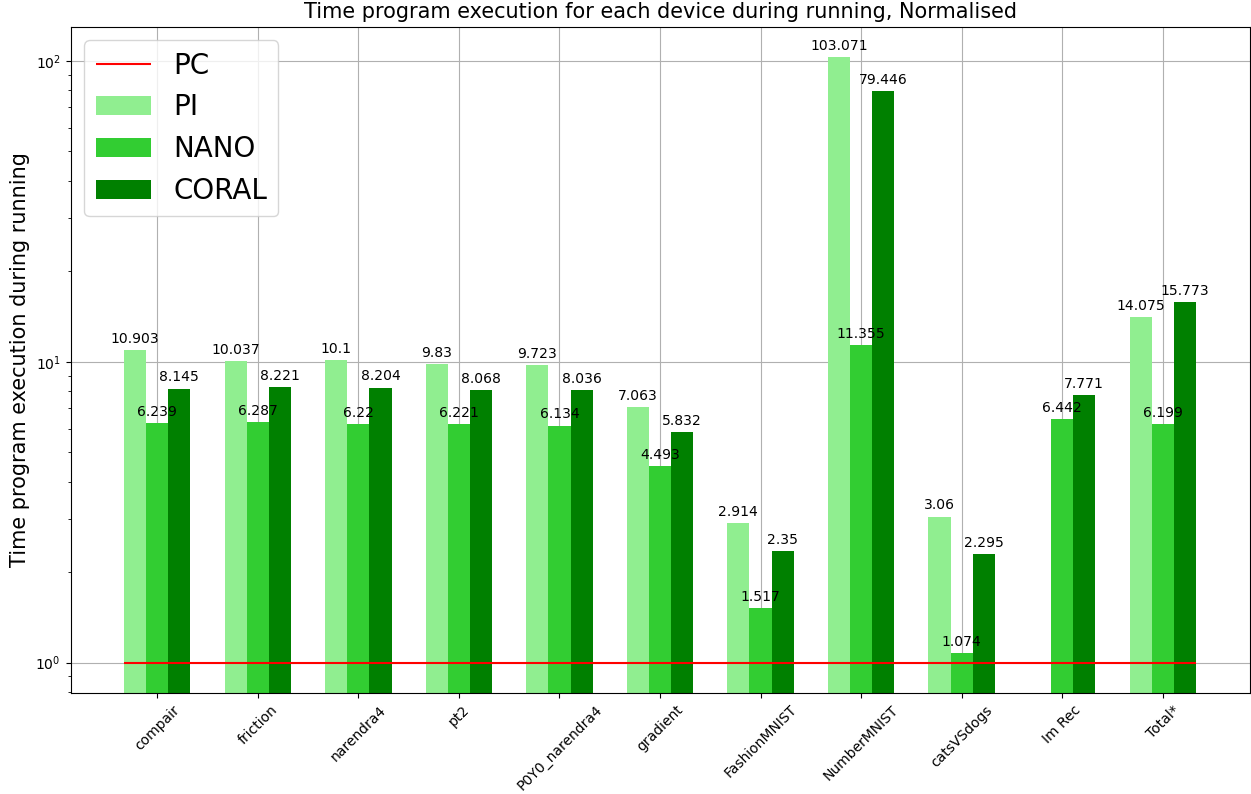
\includegraphics[width=1.25\textwidth]{afbeeldingen/Figure_2.png}}
		\caption{Staafdiagram met de genormaliseerde latencydata.}
		\label{fig:Figure_2}
	\end{figure}
	
	Beschouwen we figuur \ref{fig:Figure_1} dan kan er opgemerkt worden dat alle devices gebruik maken van ongeveer 25 \% van hun \gls{cpu}-capaciteit. Dit komt overeen met het gebruiken van \'e\'en kern in de quad-core \gls{cpu}'s. Het hogere gebruik van de \gls{cpu} bij de Personal Computer kan toegewijd worden aan de extra capaciteit die nodig is voor het aansturen van randapparatuur en -processen zoals scherm en toetsenbord, zoals ook te zien is bij $no~operations$ in de figuur.

	% wat met Im Rec  percentages die hoger liggen, catsVSdogs Pi en Coral die een beetje hoger liggen en Pi no ops op 24 %

	\begin{figure}
		\makebox[\textwidth][c]{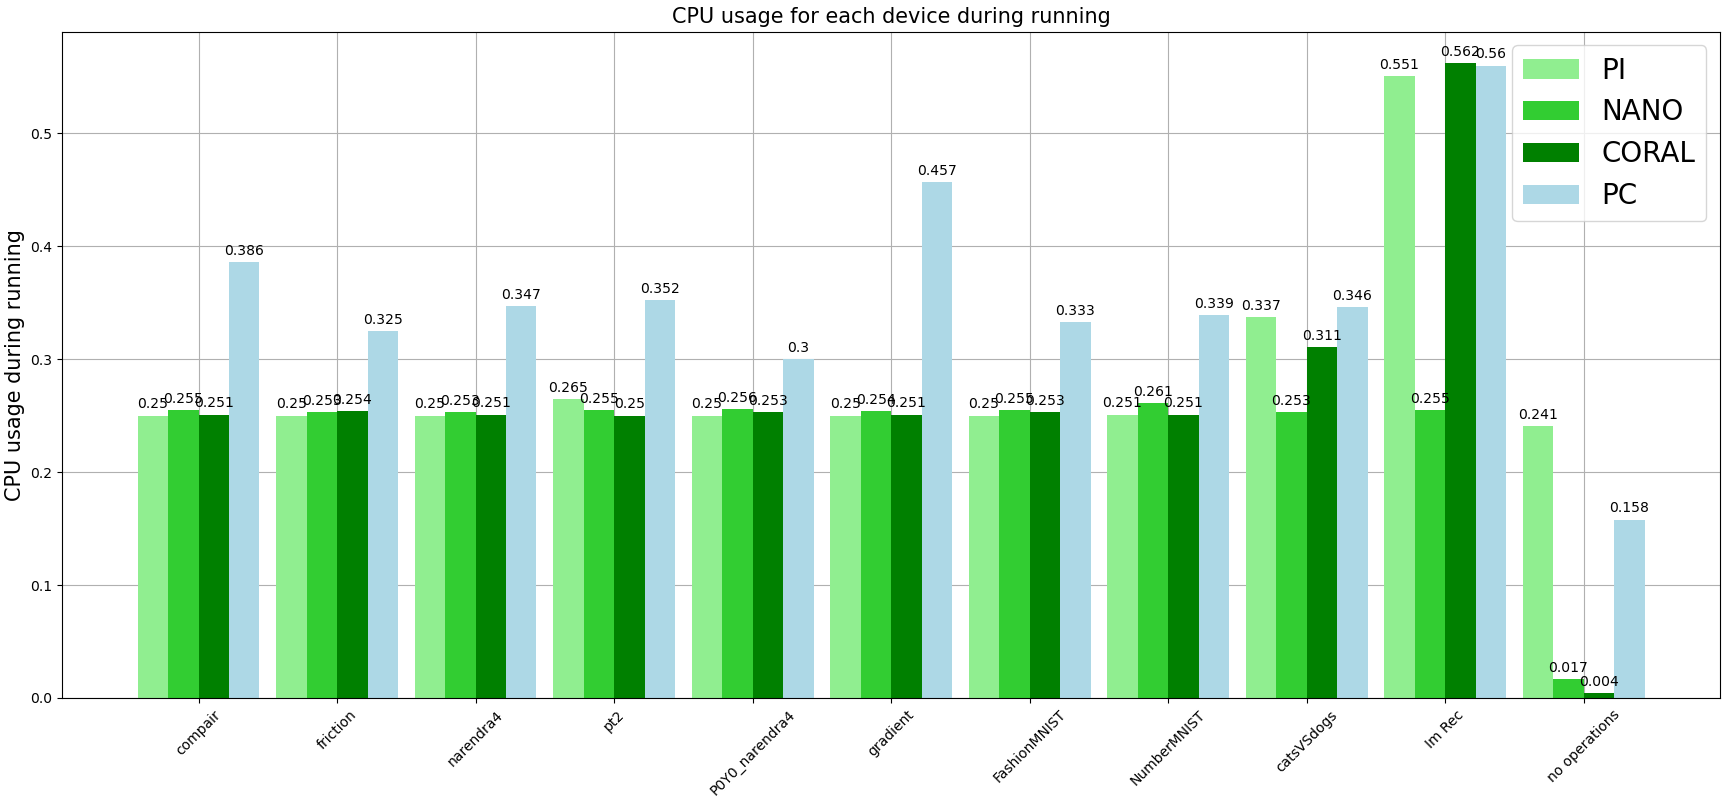
\includegraphics[width=1.25\textwidth]{afbeeldingen/Figure_1.png}}
		\caption{Staafdiagram met de CPU-verbruikgegevens.}
		\label{fig:Figure_1}
	\end{figure}

	\section{Performantie}
	De tweede analyse die gemaakt wordt, heeft betrekking tot de performantie van de toestellen die in deze thesis onderzocht worden. Hierbij worden de gegevens uit figuur \ref{fig:Figure_0} gedeeld door de gepaste kloksnelheid en percentage \gls{cpu}-gebruik zoals beschreven in hoofdstuk \ref{ch:dataverwerking}. De resultaten hiervan kan in figuur \ref{fig:Figure_3} gevonden worden. De genormaliseerde waarden zijn te vinden in figuur \ref{fig:Figure_4}.
	In het staafdiagram met de performantie van de verscheidene toestellen kunnen een aantal zaken afgeleid worden. Net zoals in vorige sectie heeft de Personal Computer de laagste waarden. Dit ligt in lijn met de hoge en performante specificaties van het toestel. Ook heeft de Jetson Nano wederom de laagste tijdwaarden tussen de verschillende edge-devices gevolgd door de Coral en met de Pi als traagste \gls{sbc}. Er kunnen gelijkaardige trends opgemerkt worden tussen figuur \ref{fig:Figure_2} en \ref{fig:Figure_4} bij de regressieprogramma's. Bij de classificatieprogramma's is een zelfde trend op te merken. Wel vinden we voor het Im Rec programma nu een andere volgorde weer. Hier presteert de Coral beter dan de Nano voor het gebruik van het mobilenet-model. Dit verschil in volgorde komt voor uit het beter gebruik van de \gls{cpu} door de Coral dan de Nano tijdens het programma Image Recognition.

	\begin{figure}
		\makebox[\textwidth][c]{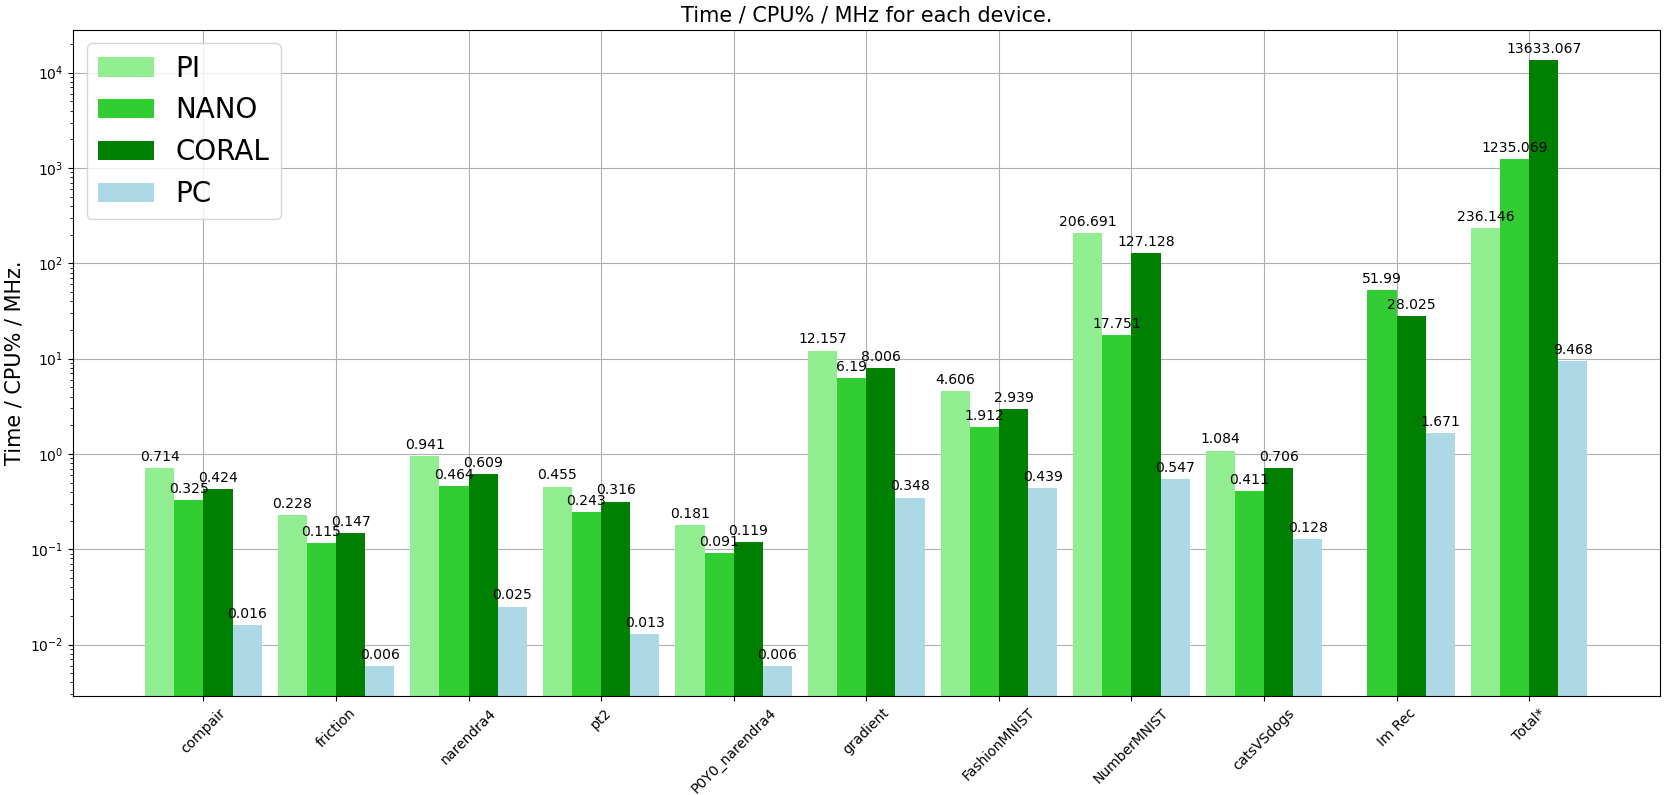
\includegraphics[width=1.25\textwidth]{afbeeldingen/Figure_3.png}}
		\caption{Staafdiagram met de performantie van de toestellen.}
		\label{fig:Figure_3}
	\end{figure}

	\begin{figure}
		\makebox[\textwidth][c]{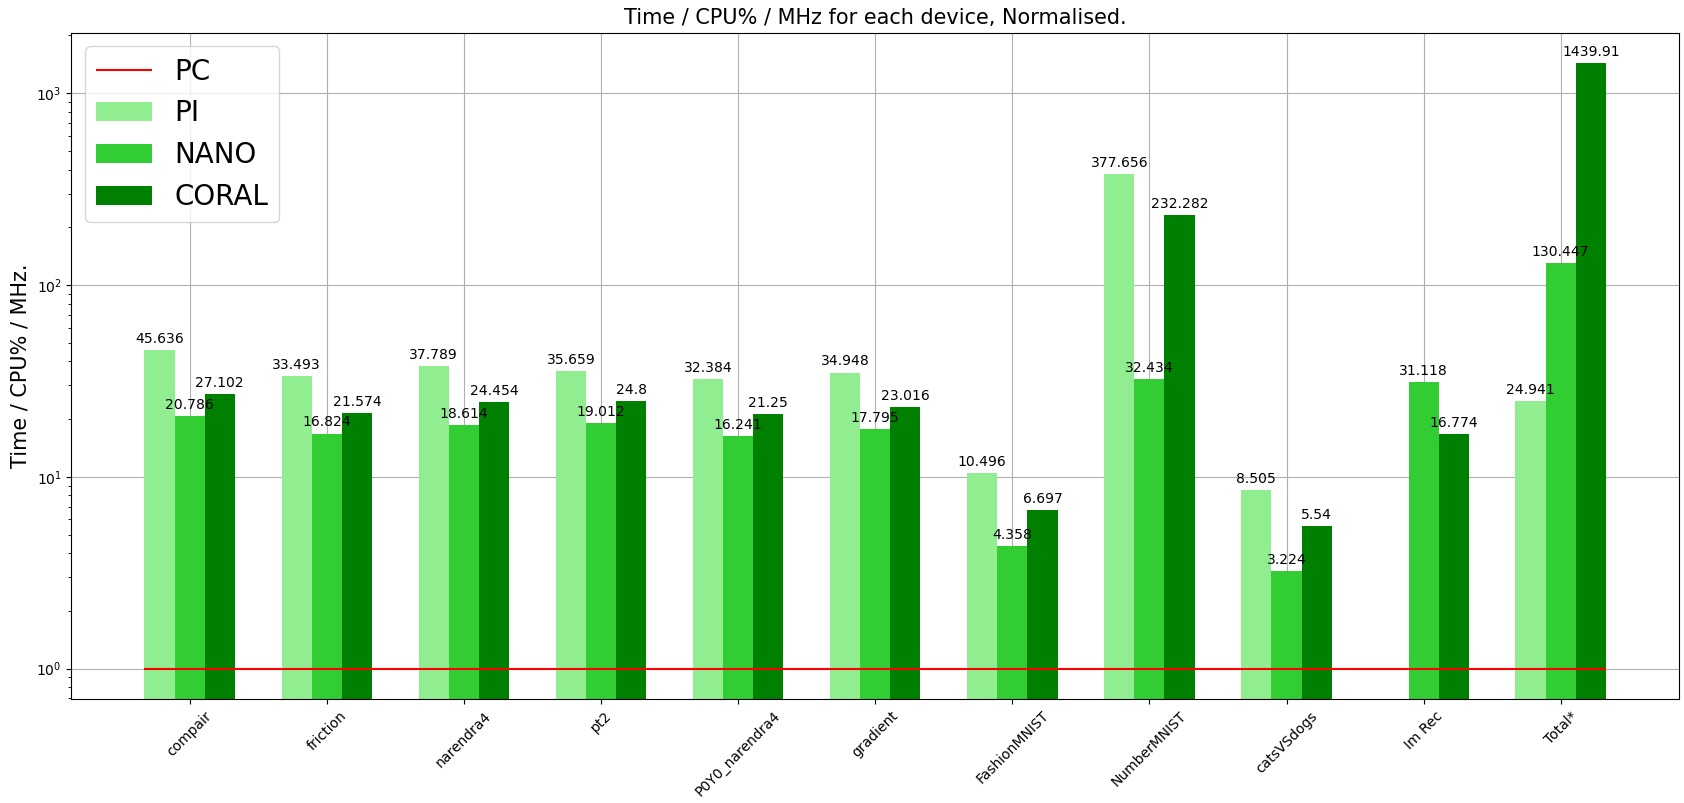
\includegraphics[width=1.25\textwidth]{afbeeldingen/Figure_4.png}}
		\caption{Staafdiagram met de genormaliseerde performantie van de toestellen.}
		\label{fig:Figure_4}
	\end{figure}

\newpage

	\section{Energieverbruik}
	Tot slot kan er ook nog een analyse gemaakt worden met betrekking tot het energieverbruik tijdens het uitvoeren van de verscheidene programma's. De resultaten hiervan kunnen in figuur \ref{fig:Figure_5} gevonden worden, de genormaliseerde waarden in figuur \ref{fig:Figure_6}. Wat opvalt bij deze figuren is dat tussen de edge devices de Nano ondanks de kortere tijdswaarden in vorige resultaten niet effici\"enter is met energie dan de andere edge-devices. De Coral Dev is over een groot deel van de programma's energie effici\"enter. Enkel bij het programma NumberMNIST en catsVSdogs verbruikt de Nano nog minder energie dan de Coral. 
	Verder vinden we ook dat de Personal Computer door de extra randapparatuur bij alle programma's behalve NumberMNIST meer verbruikt dan de verschillende \gls{sbc}s. Bij dit programma is het vooral de lange executieduur van de toestellen Raspberry Pi en de Coral Dev waardoor er meer energie verbruikt wordt. 
	
	
	\begin{figure}
		\makebox[\textwidth][c]{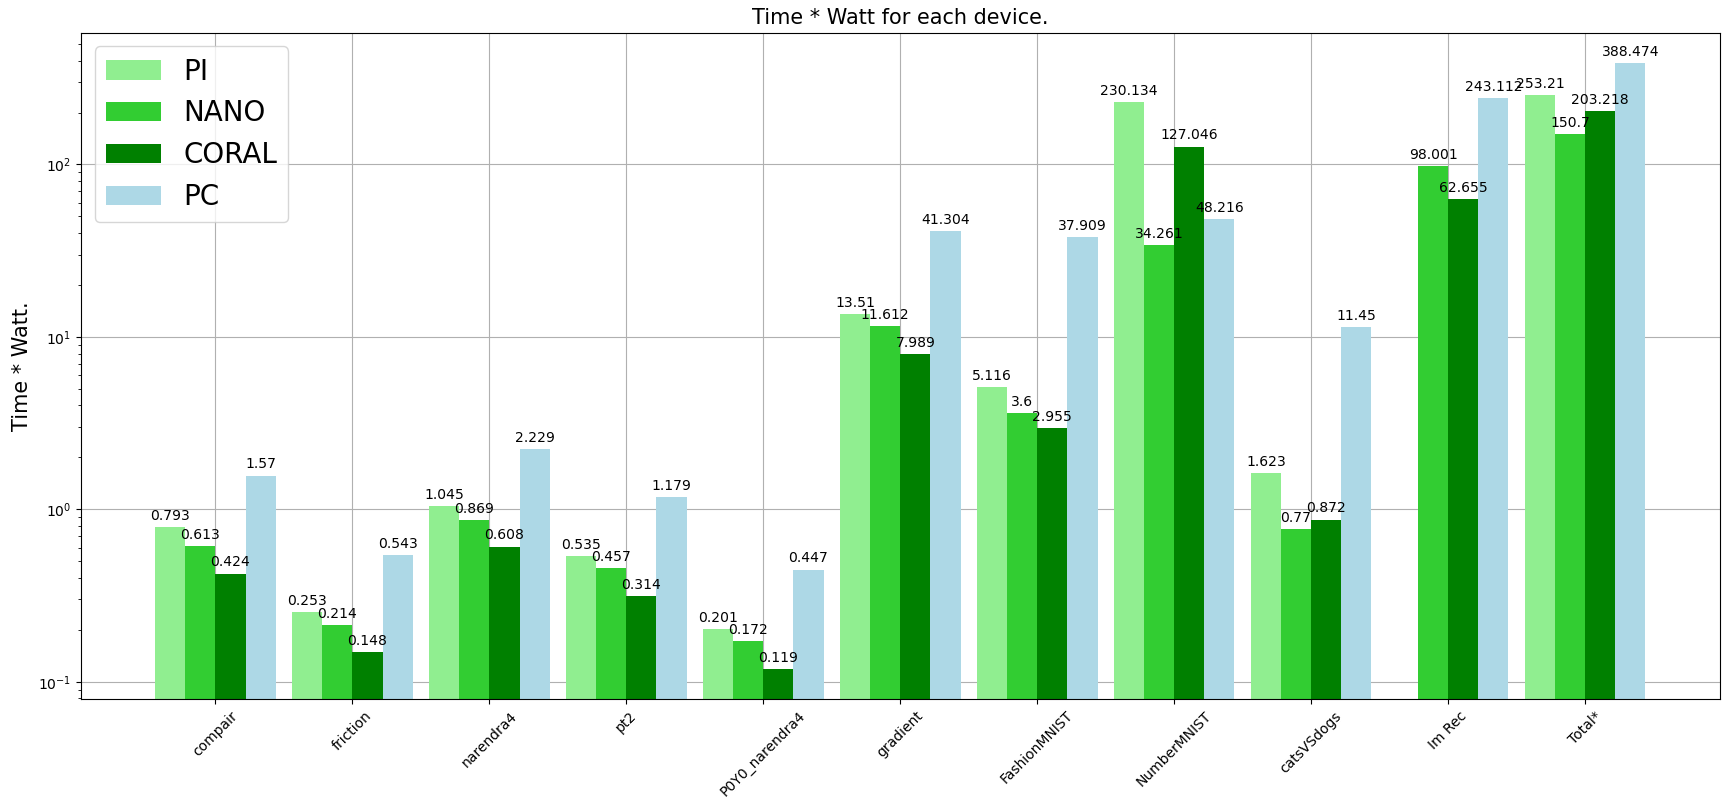
\includegraphics[width=1.25\textwidth]{afbeeldingen/Figure_5.png}}
		\caption{Staafdiagram van het energieverbruik.}
		\label{fig:Figure_5}
	\end{figure}

	\begin{figure}
		\makebox[\textwidth][c]{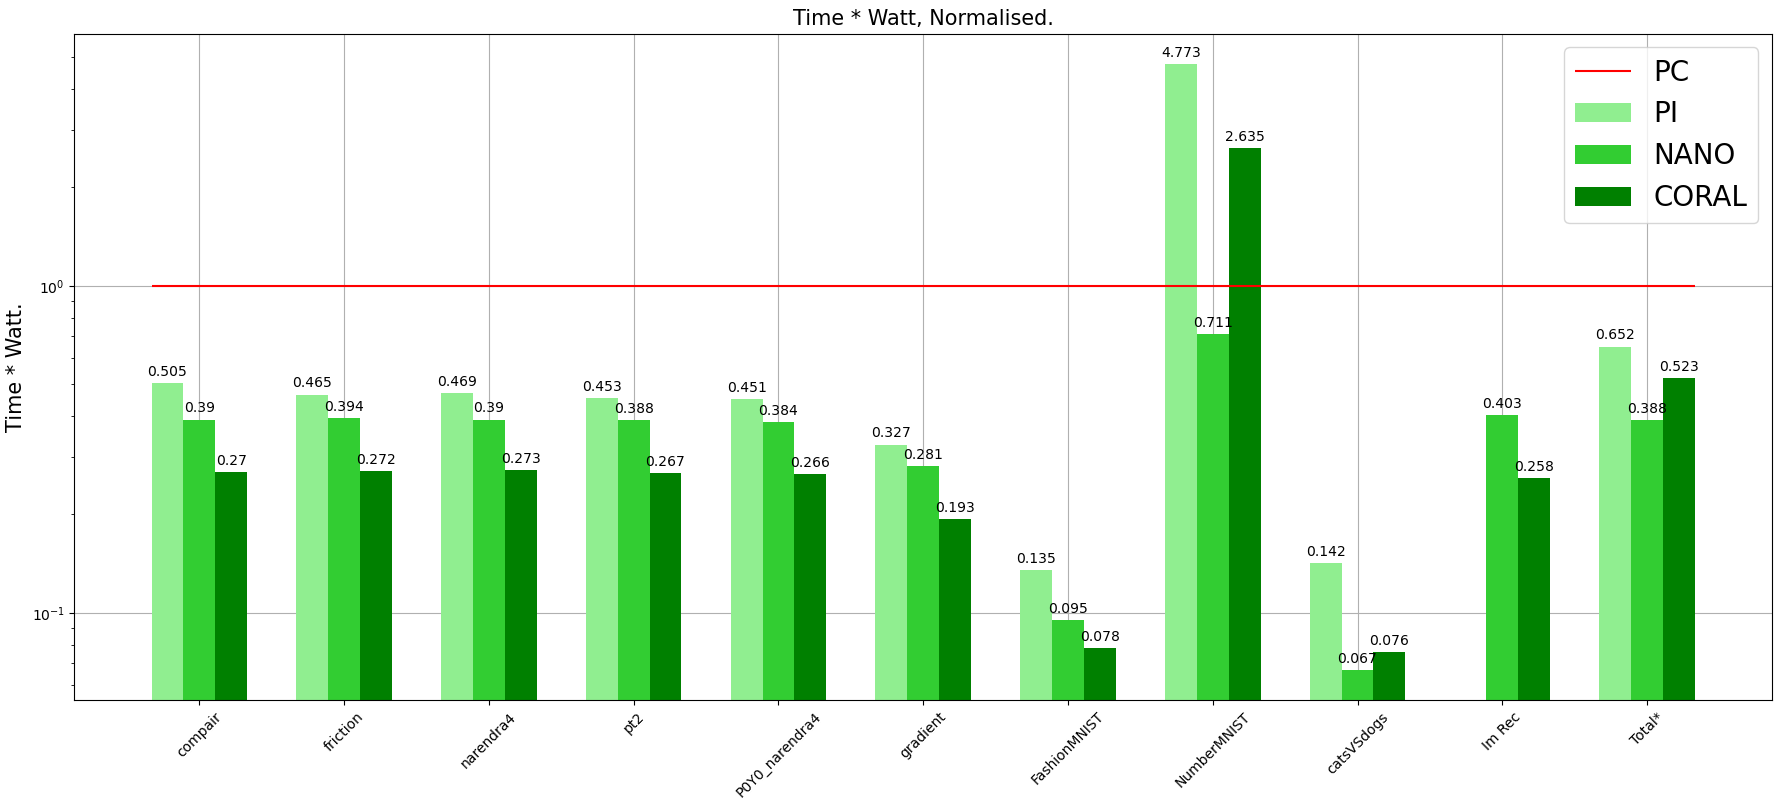
\includegraphics[width=1.25\textwidth]{afbeeldingen/Figure_6.png}}
		\caption{Staafdiagram van het genormaliseerde energieverbruik.}
		\label{fig:Figure_6}
	\end{figure}


